%! TEX program = xelatex

\documentclass{article}
\usepackage[a4paper, margin=3cm]{geometry}
\setlength{\parindent}{0pt}
\setlength{\parskip}{1em}
\usepackage{fontspec}
\setmainfont{Lato}

\usepackage{amsmath,amssymb,amsthm}
\usepackage{graphicx}
\usepackage{verbatim}
%\usepackage{pgfplots}
%\pgfplotsset{compat=1.16}

\title{}
\author{Mikael Myyrä}
\date{}

\begin{document}

\section*{1.}

Tämä on homogeeninen versio viime kerran tehtävä 3:sta hieman erilaisilla
reunaehdoilla. Nyt mukana on sekä Neumann- että Dirichlet-ehtoja.
Käytetään diskretointia
\[
  \frac{-u_{i,j-1} - u_{i-1,j} + 4u_{i,j} - u_{i+1,j} - u_{i,j+1}}{h^2} = 0.
\]
Keskeisdifferenssikaava Neumann-reunaehdoille on
\[
  \frac{u_{1,j} - 2u_{0,j} + u_{-1,j}}{2h} = 0
\]
alueen vasemmalla reunalla ja
\[
  \frac{u_{i,1} - 2u_{i,0} + u_{i,-1}}{2h} = 0
\]
alareunalla. Tähän tarvitaan haamupisteet $(i,-1)$ ja $(-1,j)$.
Laajentamalla laskenta-alue $([1, N] \times [1, N])$:stä
$([0, N] \times [0, N])$:n saadaan haamupisteiden vaikutus mukaan.

Matlab-koodi:

\verbatiminput{w4_1.m}

Lopputulos:

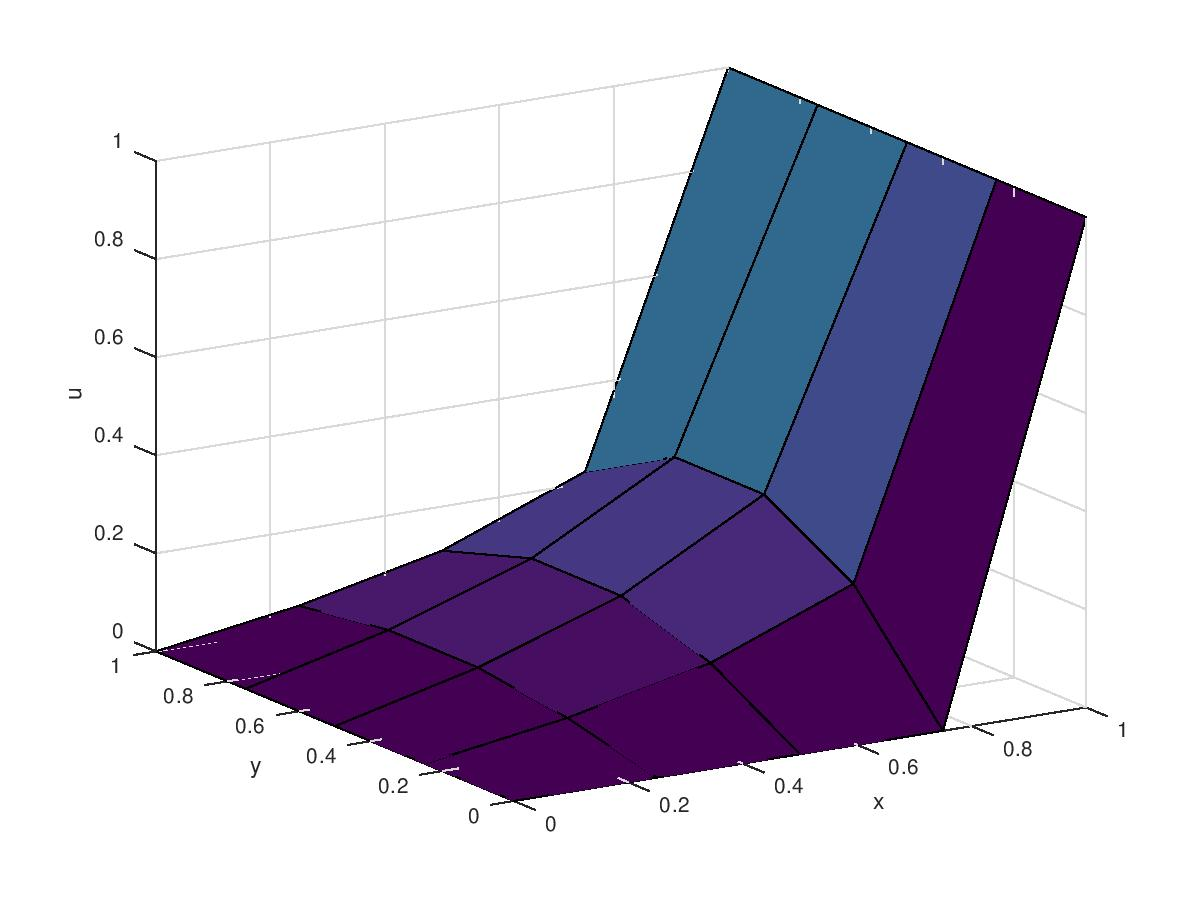
\includegraphics[width=350pt]{w4_1.jpg}

\newpage

\section*{2.}

Toteutin yhden ratkaisijan, johon voi parametrin arvolla määrätä,
käytetäänkö eksplisiittistä vai implisiittistä aika-askellusta.

Ratkaisijan koodi:

\verbatiminput{w4_heat.m}

Tämän tekemisessä paljon aikaa kului reunaehtojen ihmettelyyn ja erityisesti sen
huomaamiseen, että reunaehdon arvo piti kertoa $\alpha$:lla.

Seuraava koodi käyttää tätä ratkaisijaa tehtävään, jossa lähde on $f(x,y) =
3\sin(\pi x)\sin(\pi y)$, alkutila on $u(x,y,0) = \sin(3\pi x)\sin(3\pi y)$,
diffuusiokerroin $\alpha = 0.2$ ja reunaehdot $\frac{\partial u(0,y)}{\partial
\mathbf{n}} = \frac{\partial u(1,y)}{\partial \mathbf{n}} = 0$, $u(x,0) =
0.5\sin(\pi x)$ ja $u(x,1) = -0.5\sin(\pi x)$.  Ajassa edetään hetkeen 0.5 asti
200 askeleella.  Suoritusaikaa mitataan hilaväleillä $\frac{1}{10}$ ja
$\frac{1}{20}$ ja kuva piirretään näistä jälkimmäisellä.

\verbatiminput{w4_2.m}

Muutamalla kokeilulla hilavälillä $\frac{1}{10}$ kuluu prosessoriaikaa
eksplisiittisellä aika-askelluksella n. 0.40—0.45s ja implisiittisellä n.
1.0—1.1s.  Hilavälillä $\frac{1}{20}$ kuluu eksplisiittisellä n. 2.8—3.0s ja
implisiittisellä n. 7.1—7.3s.
Tällä pienellä otoksella implisiittinen menetelmä olisi karkeasti 2.5 kertaa hitaampi
kuin eksplisiittinen, mutta tämä ei varmasti ole lineaarinen suhde kun ratkaistavat
matriisit kasvavat suuremmiksi.

Eksplisiittisestä aika-askelluksesta huomasin kokeilemalla, että tässä käytetty
aika-askelen pituus on melko lähellä maksimia, jonka jälkeen menetelmä muuttuu
epästabiiliksi.

Kuva alkutilanteesta:

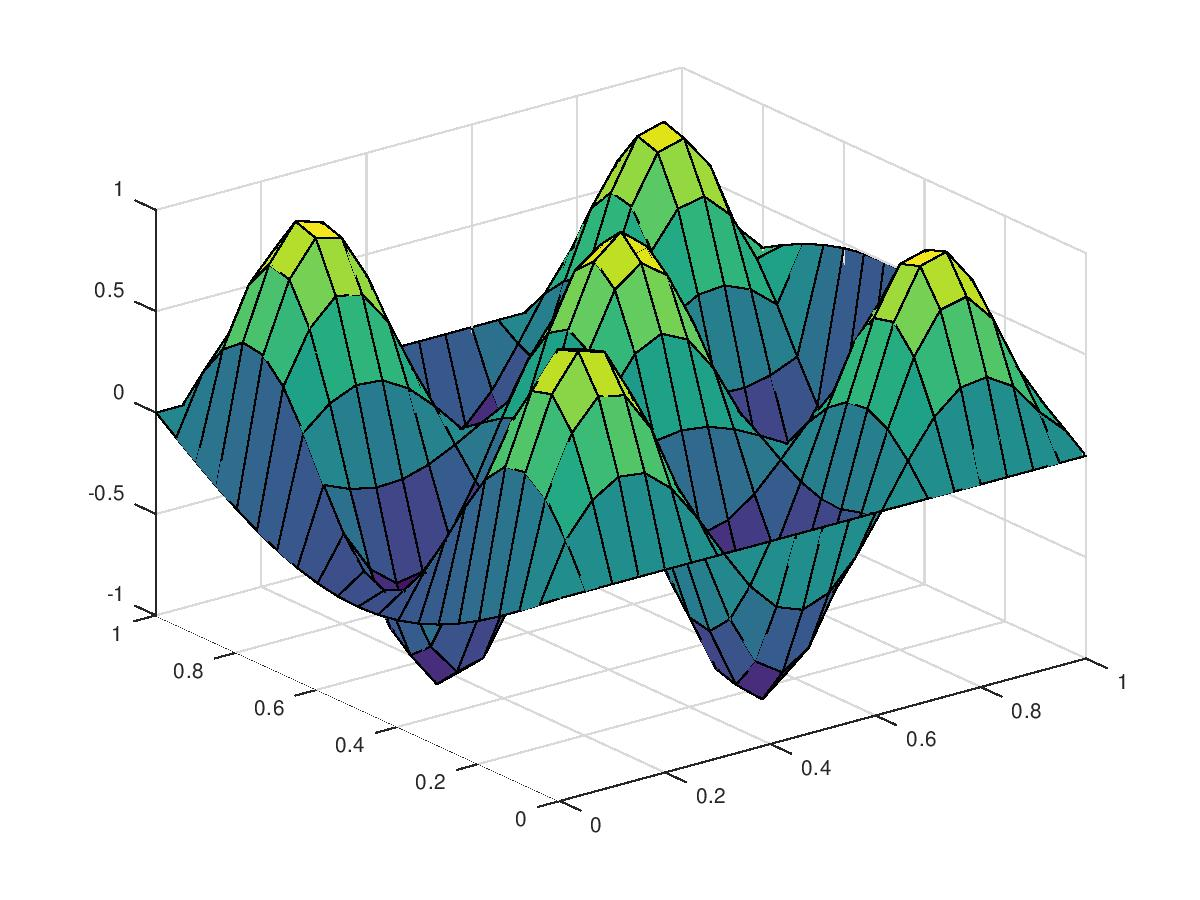
\includegraphics[width=350pt]{w4_2_start.jpg}

Ja aika-alueen lopussa:

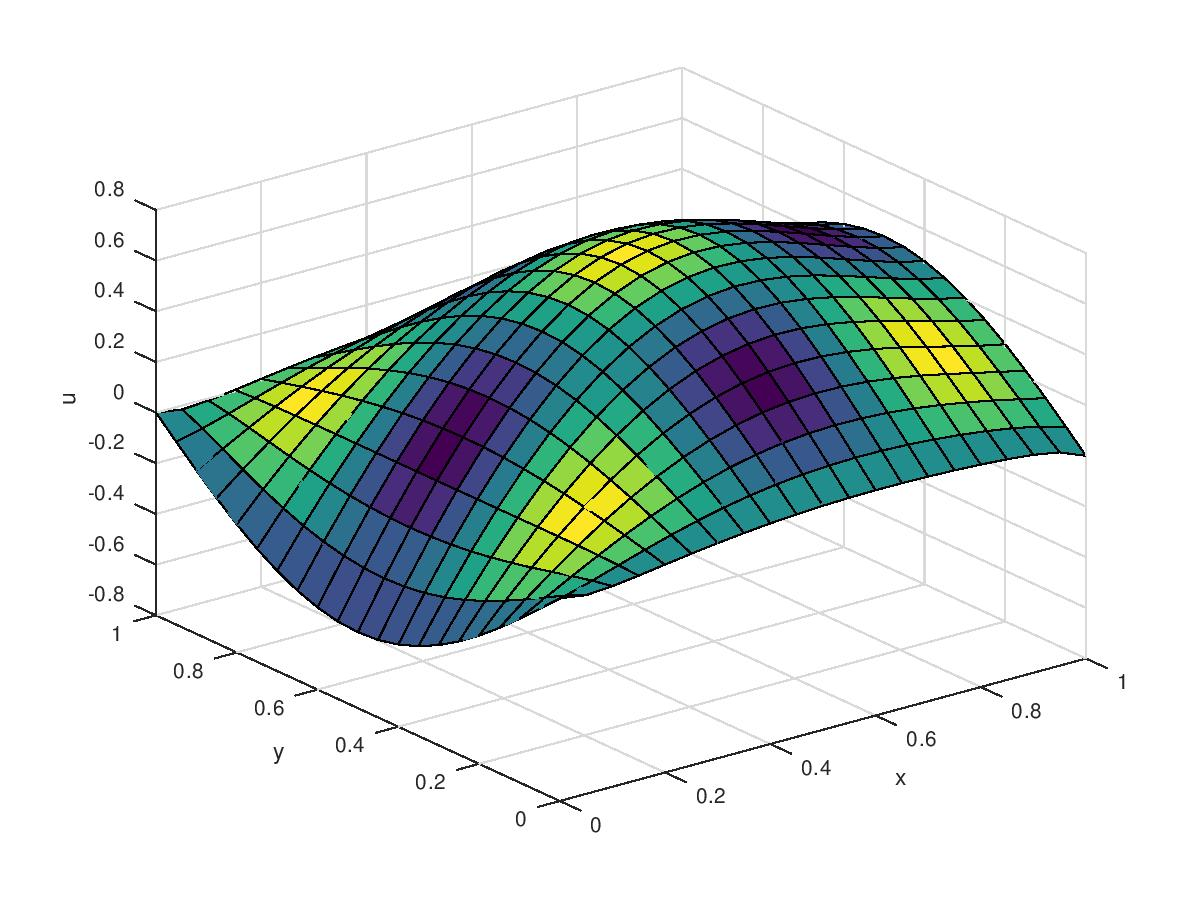
\includegraphics[width=350pt]{w4_2_end.jpg}

\newpage

\section*{3.}



\end{document}
